\chapter{Éléments de stabilité de phase} \label{ann:stabphase}
Dans le cadre de notre étude nous nous intéressons à deux phases en coexistence, une phase dite continue et l'autre dispersée. La détermination de la stabilité des phases est essentielle pour pouvoir tracer le paysage thermodynamique. La courbe binodale correspond à la condition pour laquelle deux phases peuvent coexister, c'est-à-dire que sous la courbe binodale le système peut être composé d'une seul phase, il le sera dans la zone instable et pourra l'être dans la zone métastable.
\begin{figure}[h!]
	\centering
	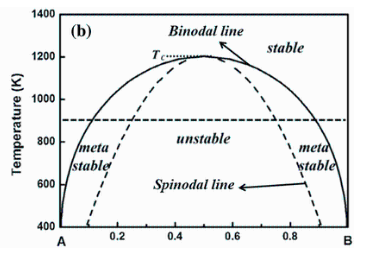
\includegraphics[width=0.5\linewidth]{figure/metastable}
	\caption[Exemple de diagramme de stabilité de phase pour un cas binaire, d'apres]{Exemple de diagramme de stabilité de phase pour un cas binaire, d'apres}
	\label{fig:metastable}
\end{figure}
Cependant le calcul de la zone instable est beaucoup plus simple que celui de la zone métastable. Pour déterminer cette zone instable on calcul la matrice Hessienne définit tel que : 
\begin{equation}
	\Mb{\doubleoverline{H}}_{g^{liq}} = \left.\frac{\partial^2 g^{liq}}{\partial \phi_i \partial \phi_j}\right|_{T,P,\phi_k\neq i,j}
	=\left.\frac{\partial^2 \Omega^{\star}}{\partial \phi_i \partial \phi_j}\right|_{T,P,\phi_k\neq i,j}
\end{equation}
L'égalité des matrices hessienne du pseudo-grand potentiel et de l'énergie libre de Gibbs est ici immédiate. D'après \cite{aursand_spinodal_2017} les zones spinodale, instable et stable sont définit tel que :
\begin{itemize}
	\item zone stable : $\displaystyle eig\left\{\Mb{\doubleoverline{H}}_{g^{liq}} \right\} > 0$, deux phases coexistent \\ 
	\item spinodale : $\displaystyle \min \left( eig \left\{\Mb{\doubleoverline{H}}_{g^{liq}}\right\} \right) > 0$, décomposition spinodale \\
	\item zone instable : $\displaystyle eig\left\{\Mb{\doubleoverline{H}}_{g^{liq}} \right\} < 0$, une phase en présence \\ 
\end{itemize}
Le calcul des valeurs propres en chaque point du paysage pouvant être coûteux on rappel que par théorème le produit des valeurs propres d'une matrice est égale au déterminant de cette matrice. Ainsi si on note $\lambda_i$ les valeurs propres de $\Mb{\doubleoverline{H}}_{g^{liq}}$ on a :
\begin{equation}
	\det{\Mb{\doubleoverline{H}}_{g^{liq}}} = \prod_i \lambda_i
\end{equation}
Pour le cas ternaire le calcul du déterminant est direct :
\begin{equation}
	\text{det}  \Mb{\doubleoverline{H}}_{g^{liq}}   =  \frac{\partial^2 g^{liq}}{\partial \phi_i^2}
	\frac{\partial^2 g^{liq}}{\partial \phi_j^2}-\left(\frac{\partial^2 g^{liq} }{\partial \phi_i \partial \phi_j} \right)^2
\end{equation}
Ainsi la zone instable correspond à la zone où le déterminant de la matrice hessienne est négatif.

